%% BioMed_Central_Tex_Template_v1.06
%%                                      %
%  bmc_article.tex            ver: 1.06 %
%                                       %

%%IMPORTANT: do not delete the first line of this template
%%It must be present to enable the BMC Submission system to
%%recognise this template!!

%%%%%%%%%%%%%%%%%%%%%%%%%%%%%%%%%%%%%%%%%
%%                                     %%
%%  LaTeX template for BioMed Central  %%
%%     journal article submissions     %%
%%                                     %%
%%          <8 June 2012>              %%
%%                                     %%
%%                                     %%
%%%%%%%%%%%%%%%%%%%%%%%%%%%%%%%%%%%%%%%%%


%%%%%%%%%%%%%%%%%%%%%%%%%%%%%%%%%%%%%%%%%%%%%%%%%%%%%%%%%%%%%%%%%%%%%
%%                                                                 %%
%% For instructions on how to fill out this Tex template           %%
%% document please refer to Readme.html and the instructions for   %%
%% authors page on the biomed central website                      %%
%% http://www.biomedcentral.com/info/authors/                      %%
%%                                                                 %%
%% Please do not use \input{...} to include other tex files.       %%
%% Submit your LaTeX manuscript as one .tex document.              %%
%%                                                                 %%
%% All additional figures and files should be attached             %%
%% separately and not embedded in the \TeX\ document itself.       %%
%%                                                                 %%
%% BioMed Central currently use the MikTex distribution of         %%
%% TeX for Windows) of TeX and LaTeX.  This is available from      %%
%% http://www.miktex.org                                           %%
%%                                                                 %%
%%%%%%%%%%%%%%%%%%%%%%%%%%%%%%%%%%%%%%%%%%%%%%%%%%%%%%%%%%%%%%%%%%%%%

%%% additional documentclass options:
%  [doublespacing]
%  [linenumbers]   - put the line numbers on margins

%%% loading packages, author definitions

\documentclass[twocolumn]{bmcart}% uncomment this for twocolumn layout and comment line below
%\documentclass{bmcart}

%%% Load packages
\usepackage{amsthm,amsmath}
%\RequirePackage{natbib}
\RequirePackage{hyperref}
\RequirePackage[authoryear]{natbib}% uncomment this for author-year bibliography
\usepackage[utf8]{inputenc} %unicode support
%\usepackage[applemac]{inputenc} %applemac support if unicode package fails
%\usepackage[latin1]{inputenc} %UNIX support if unicode package fails
\usepackage{graphicx}
\usepackage{listings}
\usepackage{color}
%%%%%%%%%%%%%%%%%%%%%%%%%%%%%%%%%%%%%%%%%%%%%%%%%
%%                                             %%
%%  If you wish to display your graphics for   %%
%%  your own use using includegraphic or       %%
%%  includegraphics, then comment out the      %%
%%  following two lines of code.               %%
%%  NB: These line *must* be included when     %%
%%  submitting to BMC.                         %%
%%  All figure files must be submitted as      %%
%%  separate graphics through the BMC          %%
%%  submission process, not included in the    %%
%%  submitted article.                         %%
%%                                             %%
%%%%%%%%%%%%%%%%%%%%%%%%%%%%%%%%%%%%%%%%%%%%%%%%%


%\def\includegraphic{}
%\def\includegraphics{}

\definecolor{listinggray}{gray}{0.1}
\definecolor{lbcolor}{rgb}{0.9,0.92,0.95}
\lstset{
	backgroundcolor=\color{lbcolor},
	tabsize=4,
	rulecolor=,
	language=Python,
        basicstyle=\scriptsize,
        %upquote=true,
        aboveskip={1.5\baselineskip},
        columns=fixed,
        showstringspaces=false,
        extendedchars=true,
        breaklines=true,
        prebreak = \raisebox{0ex}[0ex][0ex]{\ensuremath{\hookleftarrow}},
        frame=single,
        %showtabs=false,
        %showspaces=false,
        %showstringspaces=false,
        identifierstyle=\ttfamily,
        keywordstyle=\color[rgb]{0,0,1},
        commentstyle=\color[rgb]{0.133,0.545,0.133},
        stringstyle=\color[rgb]{0.627,0.126,0.941},
}

%%% Put your definitions there:
\startlocaldefs
\endlocaldefs


%%% Begin ...
\begin{document}

%%% Start of article front matter
\begin{frontmatter}

\begin{fmbox}
\dochead{Research}

%%%%%%%%%%%%%%%%%%%%%%%%%%%%%%%%%%%%%%%%%%%%%%
%%                                          %%
%% Enter the title of your article here     %%
%%                                          %%
%%%%%%%%%%%%%%%%%%%%%%%%%%%%%%%%%%%%%%%%%%%%%%

\title{scikit-image, a Python library for 2D and 3D image
processing}

%%%%%%%%%%%%%%%%%%%%%%%%%%%%%%%%%%%%%%%%%%%%%%
%%                                          %%
%% Enter the authors here                   %%
%%                                          %%
%% Specify information, if available,       %%
%% in the form:                             %%
%%   <key>={<id1>,<id2>}                    %%
%%   <key>=                                 %%
%% Comment or delete the keys which are     %%
%% not used. Repeat \author command as much %%
%% as required.                             %%
%%                                          %%
%%%%%%%%%%%%%%%%%%%%%%%%%%%%%%%%%%%%%%%%%%%%%%

\author[
   addressref={aff1},                   % id's of addresses, e.g. {aff1,aff2}
   corref={aff1},                       % id of corresponding address, if any
   %noteref={n1},                        % id's of article notes, if any
   email={emmanuelle.gouillart@saint-gobain.com}   % email address
]{\fnm{Emmanuelle} \snm{Gouillart}}
\author[
   addressref={aff2},
   %email={}
]{\fnm{Juan} \snm{Nunez-Iglesias}}
\author[
   addressref={aff3},
   email={stefanv@berkeley.edu}
]{\fnm{Stéfan} \snm{van der Walt}}



%%%%%%%%%%%%%%%%%%%%%%%%%%%%%%%%%%%%%%%%%%%%%%
%%                                          %%
%% Enter the authors' addresses here        %%
%%                                          %%
%% Repeat \address commands as much as      %%
%% required.                                %%
%%                                          %%
%%%%%%%%%%%%%%%%%%%%%%%%%%%%%%%%%%%%%%%%%%%%%%

\address[id=aff1]{%                           % unique id
  \orgname{Surface du Verre et Interfaces, UMR 125 CNRS/Saint-Gobain}, % university, etc                     %
  \postcode{93303}                                % post or zip code
  \city{Aubervilliers},                              % city
  \cny{France}                                    % country
}
\address[id=aff2]{%
  \orgname{Victorian Life Sciences Computation Initiative, University of Melbourne},
  %\street{700 Swanston St},
  %\postcode{3053}
  \city{Carlton, VIC},
  \cny{Australia}
}
\address[id=aff3]{%
  \orgname{Division of Applied Mathematics, Stellenbosch University},
  %\street{D\"{u}sternbrooker Weg 20},
  %\postcode{24105}
  \city{Stellenbosch},
  \cny{South Africa}
}



%%%%%%%%%%%%%%%%%%%%%%%%%%%%%%%%%%%%%%%%%%%%%%
%%                                          %%
%% Enter short notes here                   %%
%%                                          %%
%% Short notes will be after addresses      %%
%% on first page.                           %%
%%                                          %%
%%%%%%%%%%%%%%%%%%%%%%%%%%%%%%%%%%%%%%%%%%%%%%

%\begin{artnotes}
%\note{Sample of title note}     % note to the article
%\note[id=n1]{Equal contributor} % note, connected to author
%\end{artnotes}

\end{fmbox}% comment this for two column layout

%%%%%%%%%%%%%%%%%%%%%%%%%%%%%%%%%%%%%%%%%%%%%%
%%                                          %%
%% The Abstract begins here                 %%
%%                                          %%
%% Please refer to the Instructions for     %%
%% authors on http://www.biomedcentral.com  %%
%% and include the section headings         %%
%% accordingly for your article type.       %%
%%                                          %%
%%%%%%%%%%%%%%%%%%%%%%%%%%%%%%%%%%%%%%%%%%%%%%

\begin{abstractbox}

\begin{abstract} % abstract
\parttitle{First part title} %if any
Text for this section.

\parttitle{Second part title} %if any
Text for this section.
\end{abstract}

%%%%%%%%%%%%%%%%%%%%%%%%%%%%%%%%%%%%%%%%%%%%%%
%%                                          %%
%% The keywords begin here                  %%
%%                                          %%
%% Put each keyword in separate \kwd{}.     %%
%%                                          %%
%%%%%%%%%%%%%%%%%%%%%%%%%%%%%%%%%%%%%%%%%%%%%%

\begin{keyword}
\kwd{scikit-image}
\kwd{Python}
\kwd{image processing library}
\kwd{3-D image}
\end{keyword}

% MSC classifications codes, if any
%\begin{keyword}[class=AMS]
%\kwd[Primary ]{}
%\kwd{}
%\kwd[; secondary ]{}
%\end{keyword}

\end{abstractbox}
%
%\end{fmbox}% uncomment this for twcolumn layout

\end{frontmatter}

%%%%%%%%%%%%%%%%%%%%%%%%%%%%%%%%%%%%%%%%%%%%%%
%%                                          %%
%% The Main Body begins here                %%
%%                                          %%
%% Please refer to the instructions for     %%
%% authors on:                              %%
%% http://www.biomedcentral.com/info/authors%%
%% and include the section headings         %%
%% accordingly for your article type.       %%
%%                                          %%
%% See the Results and Discussion section   %%
%% for details on how to create sub-sections%%
%%                                          %%
%% use \cite{...} to cite references        %%
%%  \cite{koon} and                         %%
%%  \cite{oreg,khar,zvai,xjon,schn,pond}    %%
%%  \nocite{smith,marg,hunn,advi,koha,mouse}%%
%%                                          %%
%%%%%%%%%%%%%%%%%%%%%%%%%%%%%%%%%%%%%%%%%%%%%%

%%%%%%%%%%%%%%%%%%%%%%%%% start of article main body
% <put your article body there>

%%%%%%%%%%%%%%%%
%% Background %%
%%
\section*{Introduction}

The acquisition time of synchrotron tomography images has decreased
dramatically over the last decade, from hours to
seconds~\citep{Maire2014}. New modalities such as single-bunch
imaging~\citep{Rack2014} provide a time resolution down to the nanosecond
for radiography. However, the time subsequently spent in processing the
images has not decreased as much, so that the outcome of a successful
synchrotron imaging campaign often takes weeks or even months to be
transformed into scientific results. 

Transforming billions of pixels and voxels to a few meaningful figures
represents a tremendous data reduction. Often, the sequence of operations
needed to produce these data is not known beforehand, or might be altered
due to artifacts~\citep{Marone2010}, or to an unforeseen evolution of
the sample. Image processing necessarily involves trial and error phases
to choose the processing workflow. Therefore, image processing tools need
to offer at the same time enough flexibility of use, a variety of
algorithms, and efficient implementations to allow for fast iterations
while adjusting the workflow.

Several software applications and libraries are available to synchrotron
users to process their images. ImageJ~\citep{Abramoff2004, Schneider2012}
and its distribution Fiji~\citep{Schindelin2012} is a popular tool for
2-D and 3-D images, thanks to its intuitive menus and graphical tools,
and the wealth of plugins contributed by a vivid
community~\citep{Schindelin2015}. For 3-D images, commercial tools such
as Avizo 3D software (TM) are appreciated for an intuitive graphical
pipeline and advanced 3D visualization. Alternatively, the use of a
programming language gives finer control and more possibilities, provided
classical processing algorithms can be called from libraries -- hence
limiting the programming task and the risk of bugs. Matlab (TM) and its
image processing toolbox are popular in the academic community of
computer vision and image processing. The Python language is widely used
in the scientific world and in synchrotron facilities. As a
general-purpose language, Python is used in synchrotrons to control
device servers~\citep{pytango}, to reconstruct tomography volumes from
radiographs~\citep{Gursoy2014, Mirone2014}, and in data
processing packages for macromolecular cristallography~\citep{Adams2010},
azimuthal integration of diffraction data~\citep{Ashiotis2015} or
fluorescence analysis~\citep{pymca}.

\texttt{scikit-image}~\citep{Vanderwalt2014} is a general-purpose image
processing library for the Python language, and a component of the ecosystem of
Python scientific modules commonly known as Scientific
Python~\citep{Oliphant2007}. Like the rest of the ecosystem,
\texttt{scikit-image} is released under a permissive open-source license and is
available free of charge. Most of \texttt{scikit-image} is compatible with both 2-D and
3-D images, so that it can be used for a large number of imaging modalities,
such as microscopy, radiography or tomography. In this article, we explain how
\texttt{scikit-image} can be used for processing data acquired in synchrotron
imaging experiments, with a strong focus on microtomography 3-D images. This
article does not intend to be a pedagogical tutorial on \texttt{scikit-image}
for X-ray imaging, but rather to explain the rationale behind the package, and
provide various examples of its capabilities.


\section*{Overview and first steps}

In this section, we provide a short overview of the typical use patterns of
\texttt{scikit-image}, illutrated by short snippets of code. Indeed, since
Python is a programming language, the user interacts with data objects and
images through code, which is either typed and executed in an interactive
interpreter, or written in text files (scripts) that are executed. 

Images are manipulated as numerical arrays of uniform
data type, a format that guarantees a fast access to the computer memory. The
n-dimensional (2-D, 3-D, \dots) numerical array object is provided by the
\texttt{NumPy} module~\citep{Vanderwalt2011}.

In image processing, one of the first tasks is therefore to generate
\texttt{NumPy} arrays, which is often done by reading data from files. We
read one 2-D image from a file and display it with the following lines of code:

\lstinputlisting[language=Python]{io.py} 

\texttt{skimage} is the name under which \texttt{scikit-image} is imported in
Python code. Note that functions (such as \texttt{imread} to read an image
file, or \texttt{imshow} to display an image) are found in submodules of
\texttt{skimage}, such as \texttt{io}. 

A stack of 2-D images, such as tomography slices generated by a reconstruction algorithm, can be opened as an image collection or a 3-D array:
\lstinputlisting[language=Python]{io_coll.py}
Raw data formats can be opened using the \texttt{NumPy} functions \texttt{fromfile} or \texttt{memmap}, and \texttt{hdf5} files are opened using modules such as \texttt{h5py} or \texttt{pytables}.

\begin{figure*}
    \centerline{\includegraphics[width=0.8\textwidth]{ecosystem_landscape}}
\caption{\csentence{Gallery of examples of \texttt{scikit-image}.}
 The gallery of examples consists of an array of thumbnails (left part),
 which link to example webpages, each centerered on a specific image
 processing task. Each webpage includes Python code generating a figure,
 the figure itself, as well as a short tutorial explaining the image
 processing operations and the code. \label{fig:ecosystem}}
\end{figure*}



\section*{The Python ecosystem}

The benefits of \texttt{scikit-image} for image processing come not only
from the features of the package alone, but also from the rich
environment of Scientific Python~\citep{Oliphant2007, Perez2011}.
Fig.~\ref{fig:ecosystem} illustrates how several components of this
ecosystem combine into a sophisticated image processing workflow.

\paragraph{Interpreter and development environment.}

While several interpreters are available to execute interactively Python
instructions and scripts, the most popular one in the scientific world is
the IPython interpreter~\citep{Perez2007, Rossant2015}. IPython is an
advanced interpreter, which integrates syntax highlighting, text auto-completion,
a debugger,
introspection and profiling methods, and online help. Several
Integrated Development Environments (IDEs) include IPython,
together with other components such as a text editor. Notable examples
include Spyder (Fig.~\ref{fig:spyder}), PyCharm, and Visual Studio Code.

\begin{figure*}
    \centerline{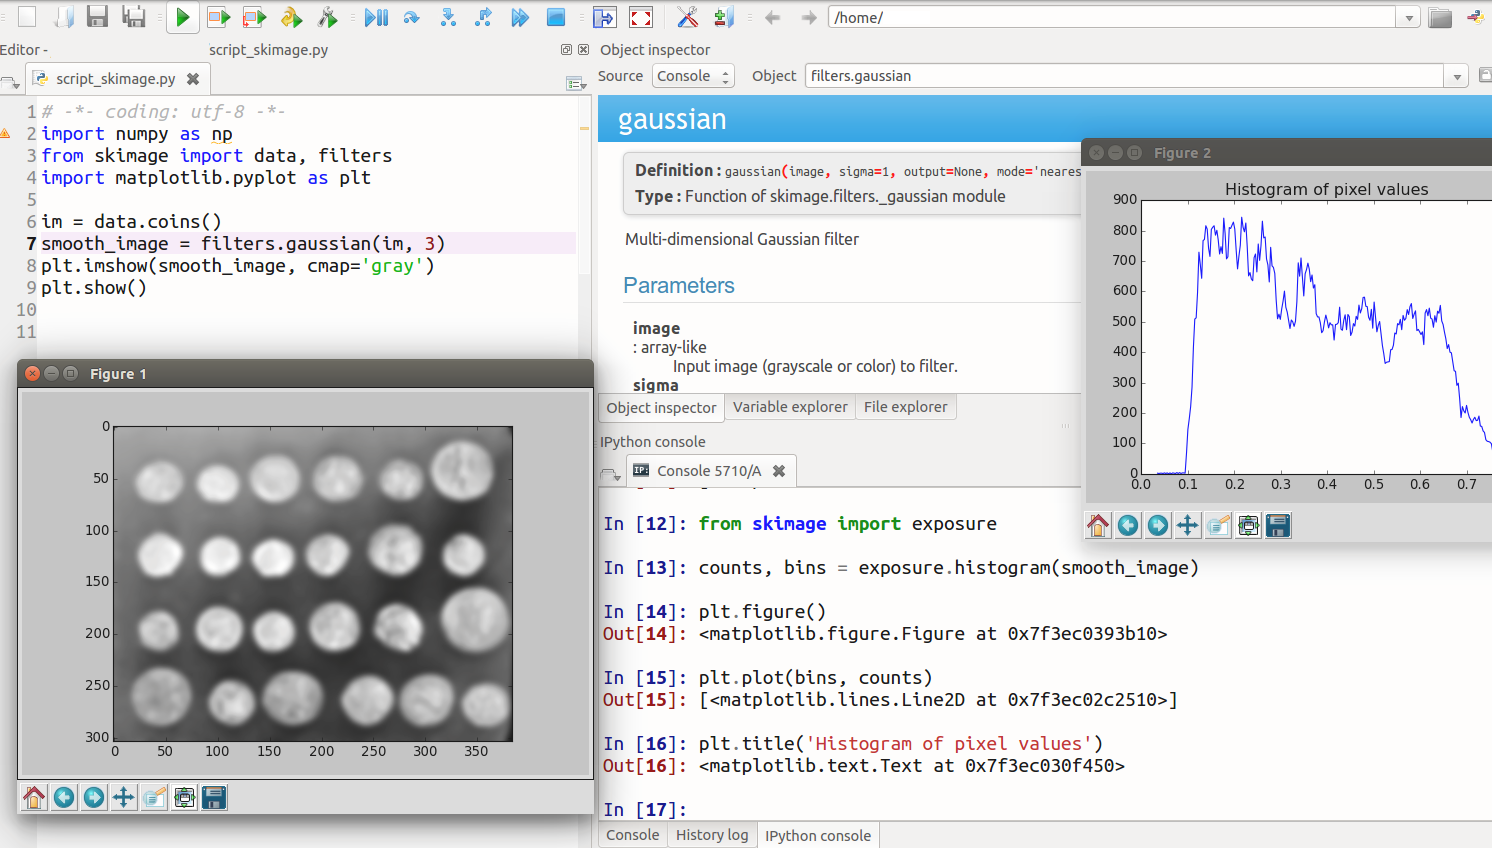
\includegraphics[width=0.99\textwidth]{spyder_process}}
\caption{\csentence{Sample figure title.}
      A short description of the figure content
  should go here. \label{fig:spyder}}
\end{figure*}

The Jupyter notebook~\citep{Kluyver2016} is a web application that grew
from the IPython project. Jupyter notebooks provide an interactive development
environment within a web browser, where live code can be enriched
by explanatory text, equations and visualizations (FIGURE).
(jni: FURTHER TEXT ABOUT IMPACT OF JUPYTER NOTEBOOKS)

\paragraph{NumPy arrays} are the cornerstone of the Scientific Python
ecosystem, and of \texttt{scikit-image} operations in particular.
Cropping or downsampling an image, or retrieving pixels corresponding to
a given label in a segmentation are all one-liners NumPy code. To
illustrate the compactness of NumPy code, modifying pixels values below a
threshold can be written as
\begin{lstlisting}
im[im < 0.5] = 0
\end{lstlisting}
using the possibility to index arrays with boolean arrays, called
\emph{masking}. Also, \texttt{NumPy} uses memory sparingly and avoids
making new copies of arrays whenever possible, which is a important
requirement when dealing with the gigabyte-sized images of tomography.
For example, cropping a subvolume as follows does not create a copy of the
original array:
\begin{lstlisting}
sub_volume = im[100:-100, 100:-100, 100:-100]
\end{lstlisting}



\paragraph{Visualization libraries.}

Visualizing images is an important component of the image processing
workflow, in order to verify the final result and to adjust the
parameters of intermediate processing operations.
\texttt{matplotlib}~\citep{Hunter2007} is the most popular 2D plotting
library of the Python ecosystem. It can be used to visualize 2D data such
as color or grayscale images, and 1D data such as contour lines, outlines
of segmented regions, histograms of gray levels, etc. Although
\texttt{matplotlib} has simple 3D plotting capabilities, we
recommend using the \texttt{mayavi} module~\citep{Ramachandran2011}
for applications requiring advanced 3D visualization, such as tomography. 
\texttt{mayavi} is based on the VTK toolkit. It exposes a simple API for
visualizing data passed as \texttt{numpy} arrays. For more advanced
visualizations, a large majority of VTK capabilities can be accessed
thanks to a pipeline API.
\texttt{mayavi} offers a good trade-off between simplicity of use for
common operations, and more advanced possibilities, including responsive
visualizations.

\paragraph{Advanced toolkits for signal processing and data science.}

\texttt{scikit-image} is only one Python module that can be used for data
processing, among many others. A very popular module is
\texttt{scikit-learn}~\citep{Pedregosa2011}, a Python module for machine
learning using \texttt{NumPy} arrays. If local features of an image
(such as local statistics of gray levels, or geometric points of
interest), or features of segmented objects (e.g. geometrical and
intensity characteristics of segmented particles) are extracted with
functions from \texttt{skimage.feature} (see Fig.~\ref{fig:ecosystem}, it
is then possible to use a \emph{classification} algorithm of
\texttt{scikit-learn}, either for labeling pixels (a segmentation task)
or to classify whole images or objects that have already been segmented.
The interoperability between these packages is ensured by the common use
of \texttt{NumPy} arrays, so that the tasks described above are
implemented with a few lines of code.

The modularity of the Scientific Python ecosystem may look
confusing at first sight. Nevertheless, core modules of this ecosystem
are almost perfectly compatible, thanks to the shared use of NumPy arrays
and common development practices (although they are developed in parallel
by different teams).


\section*{Image processing capabilities}

\begin{figure*}
    \centerline{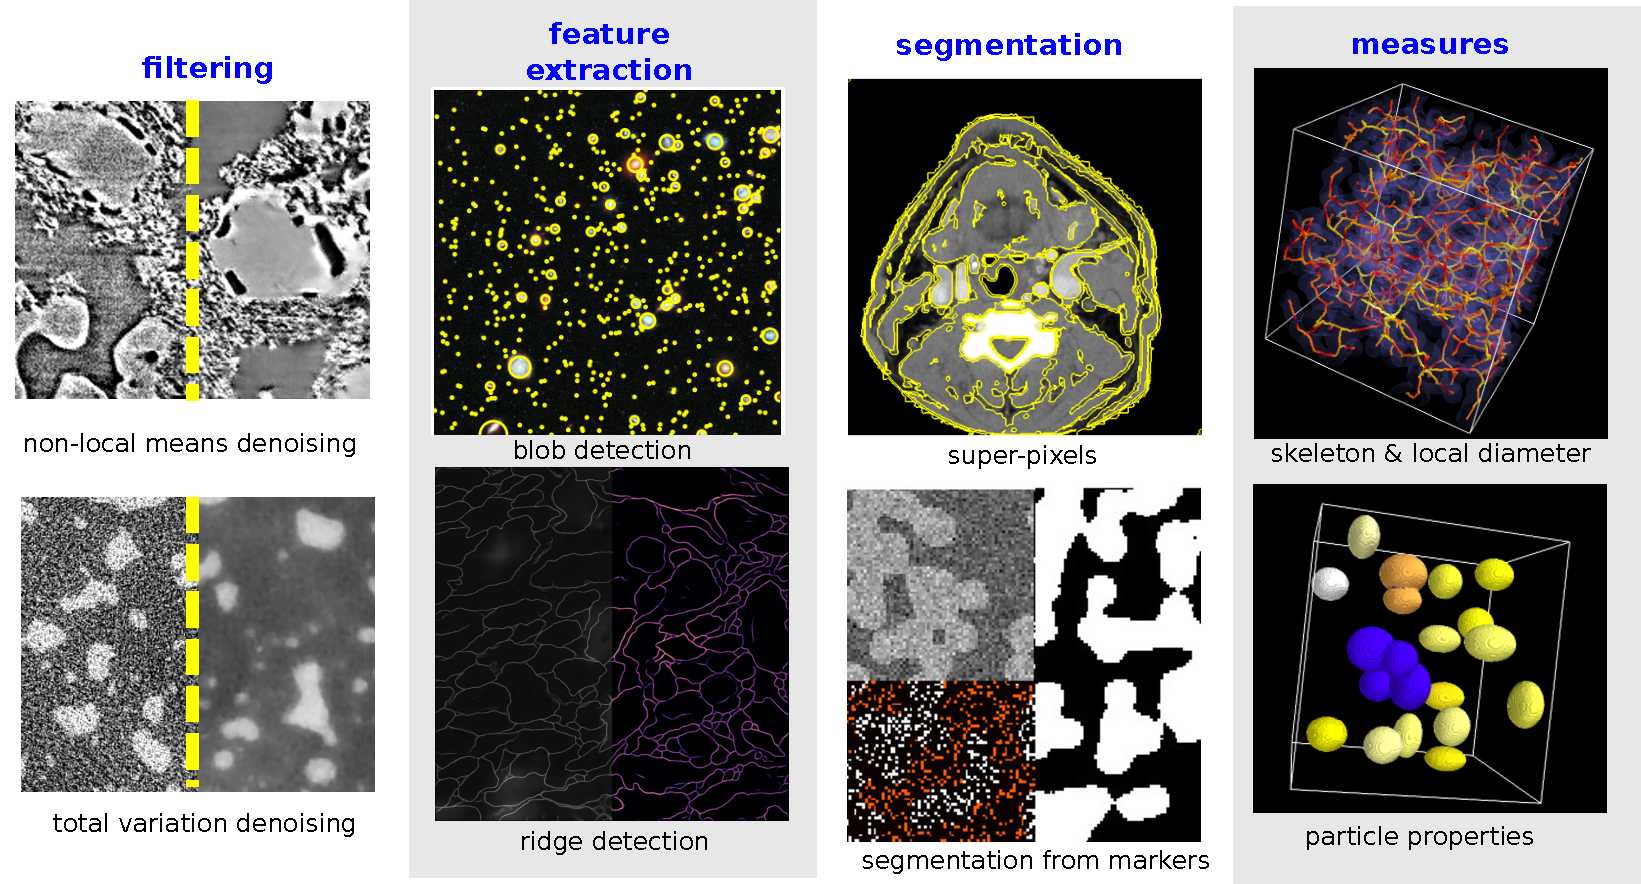
\includegraphics[width=0.99\textwidth]{tomo_gallery}}
\caption{\csentence{Sample figure title.}
      A short description of the figure content
  should go here. \label{fig:tomo_gallery}}
\end{figure*}

\texttt{scikit-image} offers all the classical operations of image
processing, such as exposure and color adjustment, filtering,
segmentation, features extraction, geometric transformations or
measurements of region characteristics. For these
different categories, the package includes both standard generic
operations and more advanced algorithms. A sample of
\texttt{scikit-image} capabilities is given in
Fig.~\ref{fig:tomo_gallery}.  

\paragraph{Performance}

\section*{Documentation and getting help}

The success of a software package aimed at end-users is strongly
correlated to the quality of its documentation (find citation).
\texttt{scikit-image} users have access to different kinds of
documentation. Functions of the API (define API here or above) are all
documented using the same standard~\citep{Pawlik2015} as other major
Scientific Python packages. The standard include a description of all
input and output variables and their data type, together with
explanations on what the function does and how to use it. Function
documentation is accessed either online, or within the development
environment (IPython, Spyder, Jupyter Notebook...). 

\begin{figure*}
    \centerline{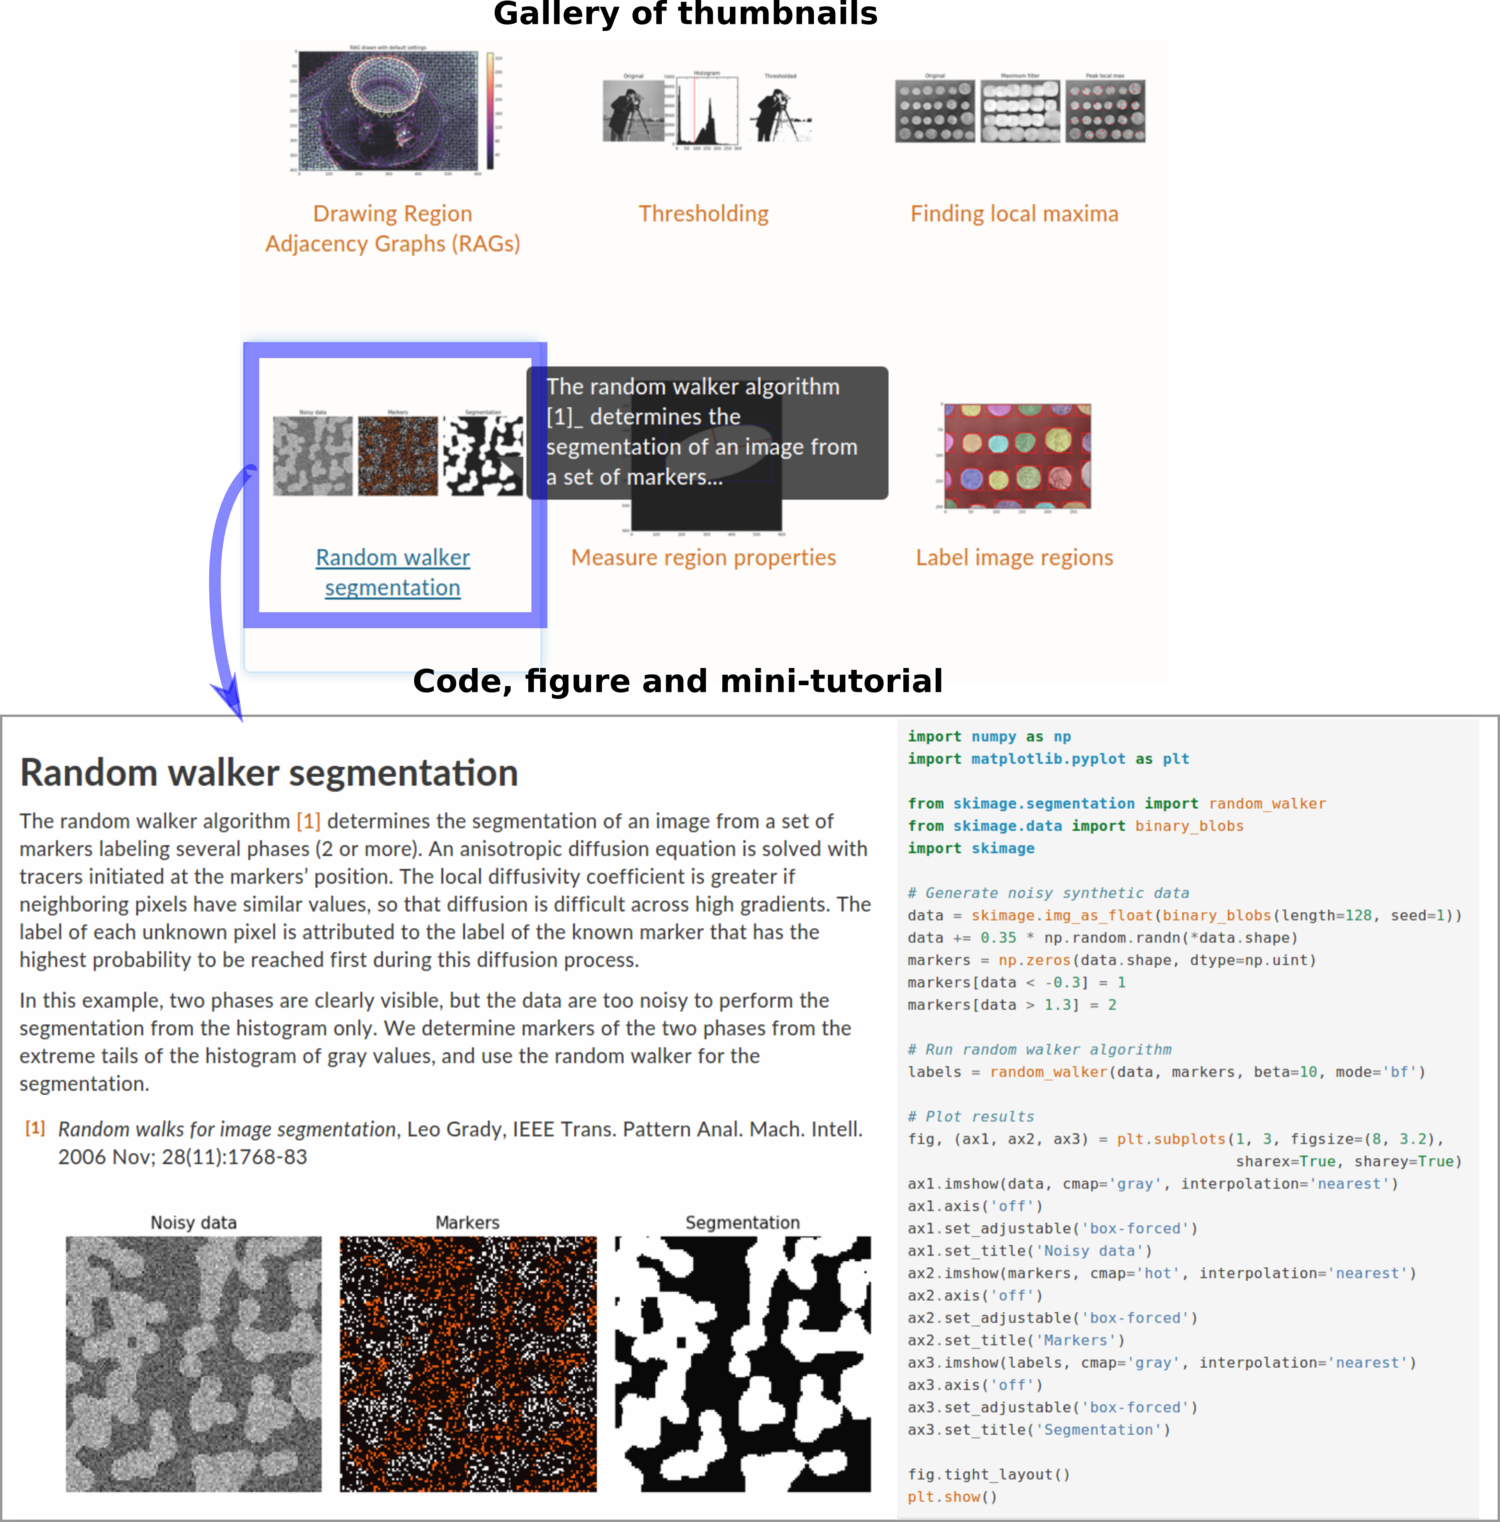
\includegraphics[width=0.99\textwidth]{figure_gallery}}
\caption{\csentence{Gallery of examples of \texttt{scikit-image}.}
 The gallery of examples consists of an array of thumbnails (left part), which link to example webpages, each centerered on a specific image processing task. Each webpage includes Python code generating a figure, the figure itself, as well as a short tutorial explaining the image processing operations and the code. \label{fig:gallery}}
\end{figure*}

In addition, a popular documentation tool is the graphical gallery of
examples (\url{http://scikit-image.org/docs/dev/auto_examples/}), a part of which is displayed in Fig.~\ref{fig:gallery}.
The principle of the gallery is to accelerate the learning curve of image
processing, by showcasing graphical examples of image processing
operations. Such examples are organized as an array of thumbnails with a
short title (see Fig.~\ref{fig:gallery} left). These thumbnails link to
the webpage of the corresponding example, which features a mini-tutorial
on the image processing method, the code needed to run the example and
the figure generated by the example. Since the graphical gallery is an
efficient way to inform users about the features of
\texttt{scikit-image}, every new feature integrated in the package must
include an example for the gallery.

Longer tutorials and a more narrative documentation is available as well
in the User Guide of \texttt{scikit-image}. The User Guide explains in
particular...

Finally, tutorials on \texttt{scikit-image} are available in various
places, either as YouTube videos, or in the SciPy Lecture
Notes~\citep{scipylecturenotes}, a comprehensive online book of Scientific
Python tutorials.  

\section*{Development and use of scikit-image}

\paragraph{Who uses scikit-image.}

Estimating the number of active users of an open-source package is a
difficult task. Statistics of downloads, for example, largely
overestimate the number of active users, all the more if the package is
bundled with others in a software distribution, like Anaconda or Canopy.
A view closer to reality can be obtained by analyzing the statistics of
visits of the online help, available on the project website.  As of the
first half of 2016, 20000 unique visitors per month visit the website of
scikit-image \url{http://scikit-image.org/}. These users come from 80
countries, located almost equally in Europe, America and Asia (Oceania
and Africa representing a much smaller fraction of visitors).

\paragraph{Development process.}

\texttt{scikit-image} is developed by a diverse team of volunteers, with
more than 170 developers that have contributed to the package. The large
number of developers and users is a key element of the sustainability of
\texttt{scikit-image}. The
development process takes place on the GitHub platform
\url{https://github.com/scikit-image/scikit-image}, where users and
developers propose and discuss new contributions, or report bugs or ideas
for improvements.
A release cycle of one or two releases every year
ensures that new features are proposed to users on a regular basis.


\section*{Conclusion}



%%%%%%%%%%%%%%%%%%%%%%%%%%%%%%%%%%%%%%%%%%%%%%
%%                                          %%
%% Backmatter begins here                   %%
%%                                          %%
%%%%%%%%%%%%%%%%%%%%%%%%%%%%%%%%%%%%%%%%%%%%%%

\begin{backmatter}

\section*{Competing interests}
: The authors declare that the research was conducted
in the absence of any commercial or financial relationships that could be
construed as a potential conflict of interest.

\section*{Acknowledgements}
  
The authors gratefully acknowledge the work of the contributors of
  \texttt{scikit-image}. E. Gouillart acknowledges the support of ANR
  project EDDAM ANR-11-BS09-027.

%%%%%%%%%%%%%%%%%%%%%%%%%%%%%%%%%%%%%%%%%%%%%%%%%%%%%%%%%%%%%
%%                  The Bibliography                       %%
%%                                                         %%
%%  Bmc_mathpys.bst  will be used to                       %%
%%  create a .BBL file for submission.                     %%
%%  After submission of the .TEX file,                     %%
%%  you will be prompted to submit your .BBL file.         %%
%%                                                         %%
%%                                                         %%
%%  Note that the displayed Bibliography will not          %%
%%  necessarily be rendered by Latex exactly as specified  %%
%%  in the online Instructions for Authors.                %%
%%                                                         %%
%%%%%%%%%%%%%%%%%%%%%%%%%%%%%%%%%%%%%%%%%%%%%%%%%%%%%%%%%%%%%

% if your bibliography is in bibtex format, use those commands:
\bibliographystyle{bmc-mathphys} % Style BST file (bmc-mathphys, vancouver, spbasic).
\bibliography{refs}      % Bibliography file (usually '*.bib' )
% for author-year bibliography (bmc-mathphys or spbasic)
% a) write to bib file (bmc-mathphys only)
% @settings{label, options="nameyear"}
% b) uncomment next line
\nocite{label}

% or include bibliography directly:
% \begin{thebibliography}
% \bibitem{b1}
% \end{thebibliography}

%%%%%%%%%%%%%%%%%%%%%%%%%%%%%%%%%%%
%%                               %%
%% Figures                       %%
%%                               %%
%% NB: this is for captions and  %%
%% Titles. All graphics must be  %%
%% submitted separately and NOT  %%
%% included in the Tex document  %%
%%                               %%
%%%%%%%%%%%%%%%%%%%%%%%%%%%%%%%%%%%

%%
%% Do not use \listoffigures as most will included as separate files

%%%%%%%%%%%%%%%%%%%%%%%%%%%%%%%%%%%
%%                               %%
%% Tables                        %%
%%                               %%
%%%%%%%%%%%%%%%%%%%%%%%%%%%%%%%%%%%

%% Use of \listoftables is discouraged.
%%
%%%%%%%%%%%%%%%%%%%%%%%%%%%%%%%%%%%
%%                               %%
%% Additional Files              %%
%%                               %%
%%%%%%%%%%%%%%%%%%%%%%%%%%%%%%%%%%%



\end{backmatter}
\end{document}
